\chapter{Matrixes} \label{app:misc}

\arraycolsep=3pt

\begin{figure}
  \begin{equation}
    \begin{array}{c | c c c c c c c c c c c c c c c c}
      Nibble	& 00 & 01 & 02 & 03 & 04 & 05 & 06 & 07 & 08 & 09 & 0A & 0B & 0C & 0D & 0E & 0F \\ \hline
      00		& 63 & 7C & 77 & 7B & F2 & 6B & 6F & C5 & 30 & 01 & 67 & 2B & FE & D7 & AB & 76 \\
      10		& CA & 82 & C9 & 7D & FA & 59 & 47 & F0 & AD & D4 & A2 & AF & 9C & A4 & 72 & C0 \\
      20		& B7 & FD & 93 & 26 & 36 & 3F & F7 & CC & 34 & A5 & E5 & F1 & 71 & D8 & 31 & 15 \\
      30		& 04 & C7 & 23 & C3 & 18 & 96 & 05 & 9A & 07 & 12 & 80 & E2 & EB & 27 & B2 & 75 \\
      40		& 09 & 83 & 2C & 1A & 1B & 6E & 5A & A0 & 52 & 3B & D6 & B3 & 29 & E3 & 2F & 84 \\
      50		& 53 & D1 & 00 & ED & 20 & FC & B1 & 5B & 6A & CB & BE & 39 & 4A & 4C & 58 & CF \\
      60		& D0 & EF & AA & FB & 43 & 4D & 33 & 85 & 45 & F9 & 02 & 7F & 50 & 3C & 9F & A8 \\
      70		& 51 & A3 & 40 & 8F & 92 & 9D & 38 & F5 & BC & B6 & DA & 21 & 10 & FF & F3 & D2 \\
      80		& CD & 0C & 13 & EC & 5F & 97 & 44 & 17 & C4 & A7 & 7E & 3D & 64 & 5D & 19 & 73 \\
      90		& 60 & 81 & 4F & DC & 22 & 2A & 90 & 88 & 46 & EE & B8 & 14 & DE & 5E & 0B & DB \\
      A0		& E0 & 32 & 3A & 0A & 49 & 06 & 24 & 5C & C2 & D3 & AC & 62 & 91 & 95 & E4 & 79 \\
      B0		& E7 & C8 & 37 & 6D & 8D & D5 & 4E & A9 & 6C & 56 & F4 & EA & 65 & 7A & AE & 08 \\
      C0		& BA & 78 & 25 & 2E & 1C & A6 & B4 & C6 & E8 & DD & 74 & 1F & 4B & BD & 8B & 8A \\
      D0		& 70 & 3E & B5 & 66 & 48 & 03 & F6 & 0E & 61 & 35 & 57 & B9 & 86 & C1 & 1D & 9E \\
      E0		& E1 & F8 & 98 & 11 & 69 & D9 & 8E & 94 & 9B & 1E & 87 & E9 & CE & 55 & 28 & DF \\
      F0		& 8C & A1 & 89 & 0D & BF & E6 & 42 & 68 & 41 & 99 & 2D & 0F & B0 & 54 & BB & 16
    \end{array}
  \end{equation}
  \caption{Rijndael S-box}
  \label{matrix:rijSbox}
\end{figure}


\begin{figure}
  \begin{equation}
    \begin{bmatrix}
      a_{1, 1} & a_{1, 2} & a_{1,3} & a_{1,4} \\
      a_{2, 1} & a_{2, 2} & a_{2,3} & a_{2,4} \\
      a_{3, 1} & a_{3, 2} & a_{3,3} & a_{3,4} \\
      a_{4, 1} & a_{4, 2} & a_{4,3} & a_{4,4}
    \end{bmatrix}
  \end{equation}
  \caption{State-Matrix}
  \label{matrix:state}
\end{figure}

\begin{figure}
  \begin{equation}
    \begin{bmatrix}
      2 & 3 & 1 & 1 \\
      1 & 2 & 3 & 1 \\
      1 & 1 & 2 & 3 \\
      3 & 1 & 1 & 2
    \end{bmatrix}
    \*
    \begin{bmatrix}
      a_{1,i} \\ 
      a_{2,i} \\
      a_{3,i} \\
      a_{4,i}
    \end{bmatrix}
    ,i = \{1,2,3,4\}
  \end{equation}
  \caption{"Rijndael MixColumns equation"}
  \label{matrix:rijMix}
\end{figure}


\begin{figure}
  \begin{center}
    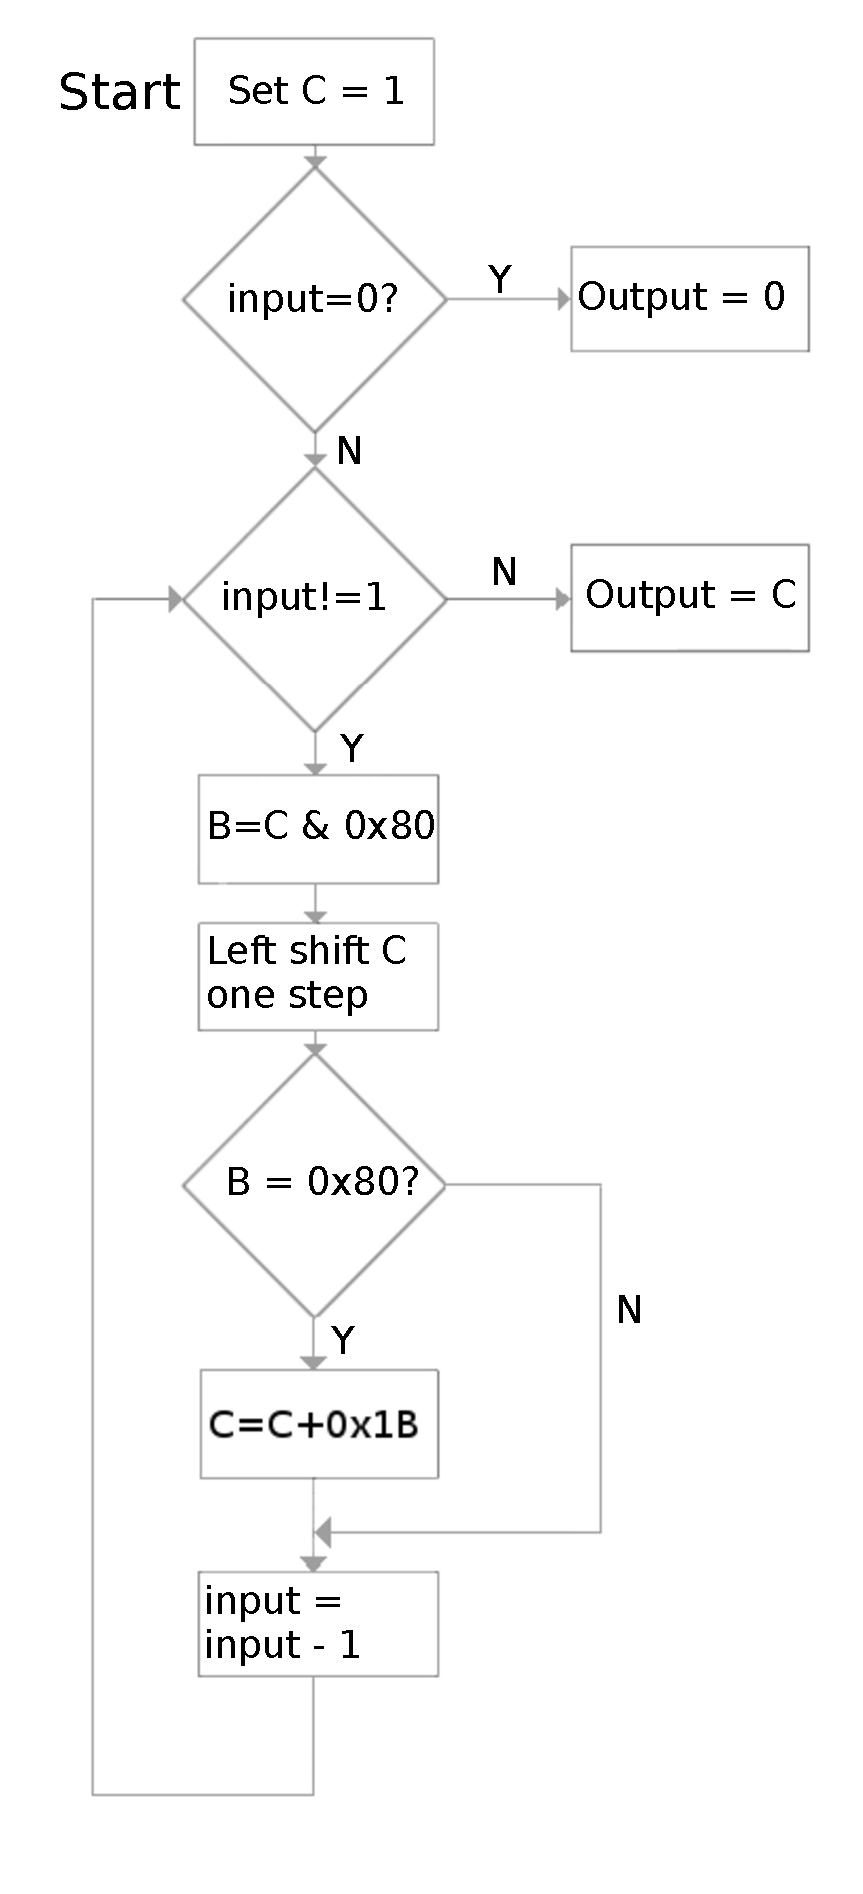
\includegraphics[height=\textheight]{flowchart}
  \end{center}
  \caption{Flowchart of the Rcon function}
  \label{app:flowchart}
\end{figure}

\begin{figure}
  \begin{center}
   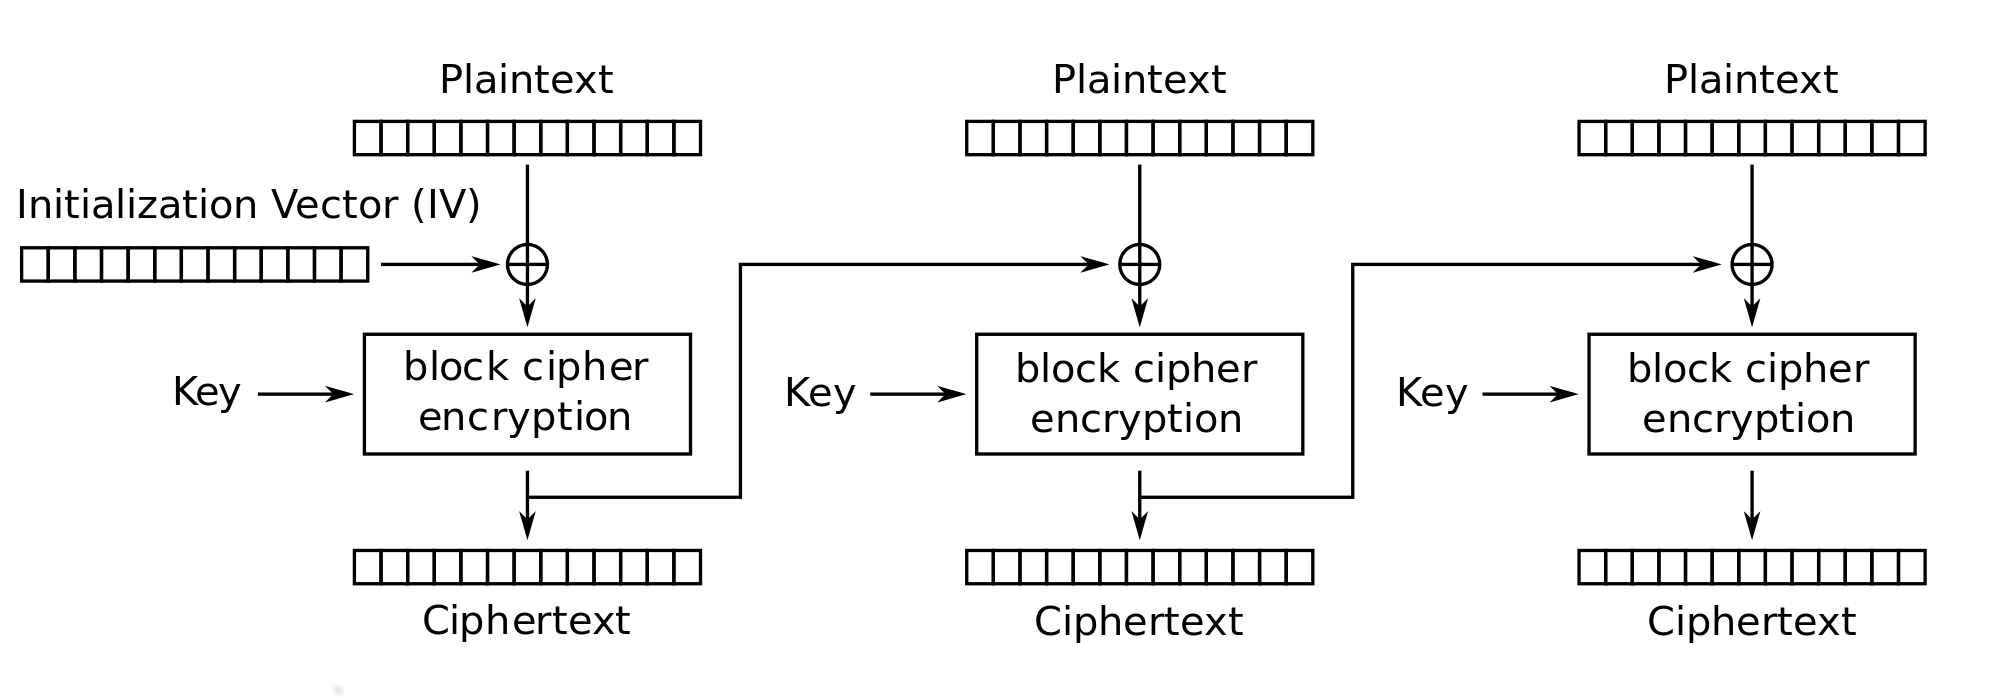
\includegraphics[width=\textwidth]{CBCmode}
  \end{center}
  \caption{Cipher block chaining mode, \citep{CBCmode:2014}}
  \label{img:CBCmode}
\end{figure}

\section{Calculations on the CBC-mode} \label{sec:CBCcalc}
The ciphertext is obtained through the following equation where \newline
C_{0} \text{ is the IV and the XOR-operation is noted with }\oplus.

C_i \text{ is the ciphertext} \newline
P_i \text{ is the plaintext} \newline
E_k \text{ is the encryption algorithm} \newline
D_k \text{ is the decryption algorithm} \newline

\begin{equation}
C_{i} = E_{k}(P_{i} \oplus C_{i-1})
\end{equation}

The inverse of the encryption algorithm E_{k} \text{ is the decryption 
algorithm } D_{k}.

The inverse of the XOR-operation the XOR-operation.

This gives us:

\begin{equation}
D_{k}(C_{i}) = P_{i} \oplus C_{i-1}
\end{equation}
which gives us
\begin{equation}
P_{i} = D_{k}(C_{i})\oplus C_{i-1}
\end{equation}
